\section{Generalized linear models}
\begin{slide}\slidetitle{Generalized linear models}
\tableofcontents[sectionstyle=show/hide,subsectionstyle=show/shaded/hide]

\end{slide}
\subsection{Generalisation of linear models}
\begin{slide}\slidetitle{Generalisation of Linear Models}

Linear models model connection between a response variable $y$ and a set $x$ of explanatory
variables by a linear dependence relation with [approximately] normal perturbations. 

\pause
\vs Many instances where either of these assumptions not appropriate, e.g.~ when the support of $y$
restricted to $\mathbb{R}_+$ or to $\mathbb{N}$.

\end{slide}\begin{slide}
\slidetitle{{\sf bank}}

Four measurements on 100 genuine Swiss banknotes and 100 counterfeit ones:
\begin{itemize}
\item[] $x_1$ length of the bill (in mm),
\item[] $x_2$ width of the left edge (in mm),
\item[] $x_3$ width of the right edge (in mm),
\item[] $x_4$ bottom margin width (in mm).
\end{itemize}

Response variable $y$: status of the banknote [$0$ for genuine and $1$ 
for counterfeit] 

\pause\vs
Probabilistic model that predicts counterfeiting based on the four measurements

\end{slide}\begin{slide}
\slidetitle{The impossible linear model}

Example of the influence of $x_4$ on $y$

Since  $y$ is binary, 
$$
y|x_4 \sim \mathscr{B}(p(x_4))\,,
$$
\MidnightBlue{{\bf \copyright~Normal model is impossible}}

\smallskip\pause
Linear dependence in $p(x)=\mathbb{E}[y|x]$'s
$$
p(x_{4i})=\beta_0+\beta_1 x_{4i}\,,
$$
\pause estimated [by MLE] as
$$
\hat p_i=-2.02+0.268\,x_{i4}
$$
which gives $\hat p_i=.12$ for $x_{i4}=8$ and ... \pause
$\hat p_i=1.19$ for $x_{i4}=12$!!!

\MidnightBlue{{\bf \copyright~Linear dependence is impossible}}

\end{slide}\begin{slide}
\slidetitle{Generalisation of the linear dependence}

Broader class of models to cover various dependence structures. 

\pause
\vs Class of {\em generalised linear models} (GLM) where
$$
y|\bx,\beta \sim f(y|\bx^\tee\beta)\,.
$$
i.e., dependence of $y$ on $\bx$ partly {\em linear} 

\end{slide}\begin{slide}
\slidetitle{Notations}

Same as in linear regression chapter, with $n$--sample
$$
\by=\left(y_1,\ldots,y_n\right)
$$ 
and corresponding explanatory variables/covariates
$$
X=\left[\begin{array}{cccc}
 x_{11} & x_{12} & \ldots & x_{1k} \\
 x_{21} & x_{22} & \ldots & x_{2k} \\
 x_{31} & x_{32} & \ldots & x_{3k} \\
 \vdots & \vdots & \vdots & \vdots \\
 x_{n1} & x_{n2} & \ldots & x_{nk}
\end{array}\right]
$$

\end{slide}\begin{slide}
\slidetitle{Specifications of GLM's}

\begin{definition}[GLM]
A GLM is a conditional model specified by two functions:
\begin{enumerate}
\item the density $f$ of $y$ given $\bx$ parameterised by its expectation parameter $\mu=\mu(\bx)$ 
[and possibly its dispersion parameter $\varphi=\varphi(\bx)$]
\pause
\item the {\em link} $g$ between the mean $\mu$ and the explanatory variables, written customarily as $g(\mu)=\bx^\tee\beta$
or, equivalently, $\mathbb{E}[y|\bx,\beta] =g^{-1}(\bx^\tee\beta)$. 
\end{enumerate}
\end{definition}

\pause
\vs For identifiability reasons, $g$ needs to be bijective. 

\end{slide}\begin{slide}
\slidetitle{Likelihood}

Obvious representation of the likelihood 
$$
\ell(\beta,\varphi|\by,X) = \prod_{i=1}^nf\left(y_i|\bx^{i\tee}\beta,\varphi\right)
$$
with parameters $\beta\in\mathbb{R}^k$ and $\varphi>0$.

\end{slide}\begin{slide}
\slidetitle{Examples}

\begin{itemize}
\item \MidnightBlue{Ordinary linear regression}

Case of GLM where 
$$
g(x)=x,\ 
\varphi=\sigma^2,\quad\text{and}\quad
\by|X,\beta,\sigma^2\sim\mathscr{N}_n(X\beta,\sigma^2).
$$
\end{itemize}

\end{slide}\begin{slide}
\slidetitle{Examples (2)}

Case of binary and binomial data, when 
$$
y_i|\bx^i\sim\mathscr{B}(n_i,p(\bx^i))
$$
with known $n_i$

\begin{itemize}
\item \MidnightBlue{Logit [or logistic regression] model}

Link is {\em logit transform} on probability of success
$$
g(p_i)=\log(p_i/(1-p_i))\,,
$$
with likelihood 
\footnotesize \begin{eqnarray*}
&& \prod_{i=1}^n\left(\begin{array}{l} n_i \\ y_i \end{array}\right)
\left(\frac{\exp(\bx^{i\tee}\beta)}{1+\exp(\bx^{i\tee}\beta)}\right)^{y_i}
\left(\frac{1}{1+\exp(\bx^{i\tee}\beta)}\right)^{n_i-y_i}\\
&&\qquad \propto \exp \left\{ \sum_{i=1}^n y_i\bx^{i\tee}\beta \right\}
\bigg/ \prod_{i=1}^n \left(1+\exp(\bx^{i\tee}\beta)\right)^{n_i-y_i}\nonumber
\end{eqnarray*}
\normalsize
\end{itemize}

\end{slide}\begin{slide}
\slidetitle{Canonical link}

Special link function $g$ that appears in the natural exponential family representation of the density
$$
g^\star(\mu)=\theta
\quad \text{if}\quad f(y|\mu)
\propto \exp \{T(y)\cdot\theta-\Psi(\theta)\}
$$

\pause
\begin{example}Logit link is canonical for the binomial model, since
$$
f(y_i|p_i) = {n_i \choose y_i}\,\exp\left\{ y_i\,\log\left( \frac{p_i}{1-p_i}\right)+n_i\,\log(1-p_i)\right\}\,, 
$$
and thus
$$
\theta_i = \log p_i/(1-p_i)
$$\end{example}

\end{slide}\begin{slide}[label=Probex]
\slidetitle{Examples (3)}

Customary to use the canonical link, but only customary ...

\begin{itemize}
\item \MidnightBlue{Probit model}

Probit link function given by
$$
g(\mu_i)=\Phi^{-1}(\mu_i)
$$
where $\Phi$ standard normal cdf

Likelihood
$$
\ell(\beta|\by,X)\propto \prod_{i=1}^n \Phi(\bx^{i\tee}\beta)^{y_i} (1-\Phi(\bx^{i\tee}\beta))^{n_i-y_i}\,.
$$

\end{itemize}\hyperlink{Proful}{\beamergotobutton{Full processing}}

\end{slide}\begin{slide}[label=LLintro]
\slidetitle{Log-linear models}

Standard approach to describe associations between several {\em categorical} 
variables, i.e, variables with finite support
 
Sufficient statistic: {\em contingency table}, made of the
cross-classified counts for the different categorical 
variables.\hyperlink{LLmdL}{\beamergotobutton{Full entry to loglinear models}}

\pause\footnotesize
\begin{example}[Titanic survivors]
{\footnotesize{\tt{\MidnightBlue{
\begin{center}\begin{tabular}{c|c|cc|cc}
\hline
        &&Child&&Adult&\\
Survivor&Class  &Male &Female &Male &Female\\
\hline
  &1st     &0      &0 &118 &4\\
  &2nd     &0      &0 &154 &13\\
No &3rd    &35     &17 &387 &89\\
  &Crew    &0      &0 &670 &3\\
\hline
  &1st     &5      &1  &57 &140\\
  &2nd    &11     &13  &14 &80\\
Yes &3rd    &13     &14  &75 &76\\
  &Crew    &0      &0  &192 &20\\
\hline
\end{tabular}\end{center}
}}}}
\end{example}\normalsize


\end{slide}\begin{slide}\slidetitle{Poisson regression model}

\begin{enumerate}
\item Each count $y_i$ is Poisson with mean $\mu_i=\mu(\bx_i)$ 
\item Link function
connecting $\mathbb{R}^+$ with $\mathbb{R}$, e.g.~logarithm
$g(\mu_i)=\log(\mu_i)$. 
\end{enumerate}

\pause\vs Corresponding likelihood 
\small
$$
\ell(\beta|y,X)=\prod_{i=1}^n\left(\frac{1}{y_i!}\right)\exp\left\{
y_i \bx^{i\tee}\beta-\exp(\bx^{i\tee}\beta)\right\}\,.
$$
\normalsize

\end{slide}\subsection{Metropolis--Hastings algorithms}\begin{slide}[label=MCMC.0]
\slidetitle{Metropolis--Hastings algorithms}

\hfill\hyperlink{Convass}{\beamergotobutton{Convergence assessment}}

\vs Posterior inference in GLMs harder than for linear models

\pause
\vs \copyright~Working with a GLM requires specific numerical or simulation tools 
[E.g., {\sf GLIM} in classical analyses] 

\pause
\vs Opportunity to introduce universal MCMC method: \MidnightBlue{{\em Metropolis--Hastings} algorithm}

\end{slide}\begin{slide}
\slidetitle{Generic MCMC sampler}

\begin{itemize}
\item Metropolis--Hastings algorithms are generic/down-the-shelf MCMC algorithms 
\item Only require likelihood up to a constant \Sepia{[difference with Gibbs sampler] }

\item can be tuned with a wide range of possibilities \Sepia{[difference with Gibbs sampler \&\ blocking]}

\item natural extensions of standard simulation algorithms: %like accept-reject or sampling-importance-resampling: 
based on the choice of a {\em proposal} 
distribution \Sepia{[difference in Markov proposal $q(x,y)$ and acceptance]}
\end{itemize}

\end{slide}\begin{slide}
\slidetitle{Why Metropolis?}

Originally introduced by Metropolis, Rosenbluth, Rosenbluth, Teller and Teller
in a setup of optimization on a discrete state-space.  All authors involved in Los Alamos during and after WWII:
\pause\small
\begin{itemize}
\item Physicist and mathematician, Nicholas Metropolis is considered (with Stanislaw Ulam) to be the father
of Monte Carlo methods. 
\item Also a physicist, Marshall Rosenbluth worked on the development of the hydrogen (H) bomb 
\item Edward Teller was one of the first scientists to work on the Manhattan Project
that led to the production of the A bomb. Also managed to design with Ulam the H bomb.
\end{itemize}\normalsize

\end{slide}\begin{slide}
\slidetitle{Generic Metropolis--Hastings sampler}

For {\em target} $\pi$ and proposal kernel $q(x,y)$

\begin{block}{\sffamily
\begin{itemize}
\small
\item[ ] {\bfseries Initialization:} Choose an arbitrary $x^{(0)}$
\pause
\item[ ] {\bfseries Iteration $t$:} 
\normalsize
\begin{enumerate}
\item Given $x^{(t-1)}$, generate $\tilde x \sim q(x^{(t-1)},x)$
\item Calculate 
$$
\rho(x^{(t-1)},\tilde x)=\min\left(\frac{\pi(\tilde x)/q(x^{(t-1)},\tilde x)}{\pi(x^{(t-1)})/q(\tilde x,x^{(t-1)})},1\right)
$$
\item  With probability $\rho(x^{(t-1)},\tilde x)$ accept $\tilde x$ and set $x^{(t)}=\tilde x$;\\
otherwise reject $ \tilde x$ and set $x^{(t)}=x^{(t-1)}$.
\end{enumerate}
\end{itemize}
}\end{block}

\end{slide}\begin{slide}
\slidetitle{Universality}

Algorithm only needs to simulate from 
$$q$$ which can be chosen [almost!] arbitrarily, i.e.~unrelated with $\pi$ 
[$q$ also called {\em instrumental} distribution]

\vs
{\bf Note:} $\pi$ and $q$ known up to proportionality terms ok since proportionality constants cancel in $\rho$. 

\end{slide}\begin{slide}
\slidetitle{Validation}

\begin{block}{Markov chain theory}
Target $\pi$ is stationary distribution of Markov chain $(x^{(t)})_t$ because
probability $\rho(x,y)$ satisfies \BurntOrange{{\em detailed balance equation}}
$$
\pi(x) q(x,y) \rho(x,y) = \pi(y) q(y,x) \rho(y,x)
$$
{\em [Integrate out $x$ to see that $\pi$ is stationary]}
\end{block}

\vs\pause
For convergence/ergodicity, Markov chain must be {\em irreducible}: $q$ has positive probability of reaching all areas 
with positive $\pi$ probability in a finite number of steps.

\end{slide}\begin{slide}
\slidetitle{Choice of proposal}

Theoretical guarantees of convergence very high, but choice of $q$ is crucial in practice. \pause
Poor choice of $q$ may result in 
\begin{itemize}
\item very high rejection rates, with very few moves of the Markov 
chain $(x^{(t)})_t$ hardly moves, or in 
\pause
\item a myopic exploration of the support of $\pi$, that is, in a dependence on
the starting value $x^{(0)}$, with the chain stuck in a neighbourhood mode to $x^{(0)}$.
\end{itemize}

\pause
\begin{block}{Note: hybrid MCMC}
Simultaneous use of different kernels valid {\em and} recommended
\end{block}

\end{slide}\begin{slide}
\slidetitle{The independence sampler}

Pick proposal $q$ that is independent of its first argument,
$$
q(x,y)=q(y)
$$
$\rho$ simplifies into
$$
\rho(x,y)=\min\left(1,\frac{\pi(y)/q(y)}{\pi(x)/q(x)}\right)\,.
$$

\begin{block}{Special case: $q\propto\pi$}
Reduces to $\rho(x,y)=1$ and iid sampling
\end{block}

\pause Analogy with Accept-Reject algorithm where $\max \pi/q$
replaced with the current value $\pi(x^{(t-1)})/q(x^{(t-1)})$ 
but sequence of accepted $x^{(t)}$'s not i.i.d.

\end{slide}\begin{slide}
\slidetitle{Choice of $q$}

Convergence properties highly dependent on $q$. 
\begin{itemize}
\item $q$ needs to be positive everywhere on the support of $\pi$
\item for a good exploration of this support, $\pi/q$ needs to be bounded. 
\end{itemize}

\vs\pause Otherwise, the chain takes too long to reach regions with low $q/\pi$ values. 

\end{slide}\begin{slide}
\slidetitle{The random walk sampler}

Independence sampler requires too much global information about $\pi$:
opt for a local gathering of information

\vs\pause Means exploration of the neighbourhood of the current value $x^{(t)}$
in search of other points of interest. 

\vs\pause Simplest exploration device is based on random walk dynamics.\\

\end{slide}\begin{slide}
\slidetitle{Random walks}

Proposal is a symmetric transition density 
$$
q(x,y)=q_{RW}(y-x)=q_{RW}(x-y)
$$

\vs\pause Acceptance probability $\rho(x,y)$ reduces to the simpler form
$$
\rho(x,y)=\min\left(1,\frac{\pi(y)}{\pi(x)}\right)\,.
$$
Only depends on the target $\pi$ 
{\em [accepts all proposed values that increase $\pi$]}

\end{slide}\begin{slide}
\slidetitle{Choice of $q_{RW}$}

Considerable flexibility in the choice of $q_{RW}$,
\begin{itemize}
\item tails: Normal versus Student's $t$
\item scale: size of the neighbourhood 
\end{itemize}

\vs\pause 
Can also be used for restricted support targets [with a waste of simulations near the boundary]

\vs\pause
Can be tuned towards an acceptance probability of $0.234$ at the {\em burnin} stage 
\Sepia{{\em [Magic number!]}}

\end{slide}\begin{slide}[label=Convass]
\slidetitle{Convergence assessment}

\BurntOrange{{\bf Capital question: How many iterations do we need to run???}}
\hfill\hyperlink{MCMC.0}{\beamerreturnbutton{MCMC debuts}}

\pause
\begin{itemize}
\item \MidnightBlue{{\bf Rule \# 1}} There is no absolute number of simulations, i.e.
$1,000$ is neither large, nor small.
\item \MidnightBlue{{\bf Rule \# 2}} It takes [much] longer to check for convergence 
than for the chain itself to converge.
\item \MidnightBlue{{\bf Rule \# 3}} MCMC is a {\em ``what-you-get-is-what-you-see"} algorithm: it 
fails to tell about unexplored parts of the space.
\item \MidnightBlue{{\bf Rule \# 4}} When in doubt, run MCMC chains in parallel and check for 
consistency.
\end{itemize}
\vs\pause
Many ``quick-\&-dirty" solutions in the literature, but not necessarily trustworthy.

\end{slide}\begin{slide}
\slidetitle{Prohibited dynamic updating}

\begin{itemize}
\item[$\lightning$] \MidnightBlue{
Tuning the proposal in terms of its past performances can only
be implemented at {\em burnin}, because otherwise this cancels Markovian convergence 
properties.}
\end{itemize}

\vs\pause
Use of several MCMC proposals together within a single
algorithm using circular or random design is ok.
It almost always brings an improvement compared with its individual components (at the cost
of increased simulation time)

\end{slide}
\begin{slide}\slidetitle{Effective sample size}

\Sepia{{\bf How many iid simulations from
$\pi$ are equivalent to $N$ simulations from the MCMC algorithm?}}

\vs\pause
Based on estimated $k$-th order auto-correlation,
$$
\rho_k = \mathrm{corr}\left(x^{(t)},x^{(t+k)} \right)\,,
$$
effective sample size
\small$$
N^\text{ess} = n\,\left(1+2\,\sum_{k=1}^{T_0} \hat\rho_k^2\right)^{-1/2}\,,
$$\normalsize
\begin{enumerate}
\item[{\Large $\lightning$}] Only partial indicator that fails to signal
chains stuck in one mode of the target 
\end{enumerate}

\end{slide}\subsection{The Probit Model}\begin{slide}[label=Proful]
\slidetitle{The Probit Model}

Likelihood\hyperlink{Probex}{\beamerreturnbutton{Recall Probit}}
$$
\ell(\beta|\by,X)\propto \prod_{i=1}^n \Phi(\bx^{i\tee}\beta)^{y_i} (1-\Phi(\bx^{i\tee}\beta))^{n_i-y_i}\,.
$$

\pause If no prior information available, resort to the flat prior 
$\pi(\beta)\propto 1$ and then obtain the posterior distribution
$$
\pi(\beta|\by,X) \propto \prod_{i=1}^n \Phi\left(\bx^{i\tee}\beta\right)^{y_i}\left(1-\Phi(\bx^{i\tee}\beta)\right)^{n_i-y_i}\,,
$$
nonstandard and simulated using MCMC techniques.

\end{slide}\begin{slide} 
\slidetitle{MCMC resolution}

\vs Metropolis--Hastings random walk sampler works well for binary regression problems with
small number of predictors

\vs Uses the maximum likelihood estimate
$\hat\beta$ as starting value and asymptotic (Fisher)
covariance matrix of the MLE, $\hat\Sigma$, as scale

\end{slide}
\begin{frame}[fragile]
\frametitle{MLE proposal}

{\sf R} function {\sf glm} very useful to get the maximum likelihood estimate of $\beta$ 
and its asymptotic covariance matrix $\hat\Sigma$.

\vs Terminology used in {\sf R} program\small
\begin{verbatim}
mod=summary(glm(y~X-1,family=binomial(link="probit")))
\end{verbatim}\normalsize 
with {\sf mod{\$}coeff[,1]} denoting $\hat\beta$ and {\sf mod{\$}cov.unscaled} $\hat\Sigma$.

\end{frame}
\begin{slide}
\slidetitle{MCMC algorithm}

\begin{block}{Probit random-walk Metropolis-Hastings}
\begin{itemize}{\sffamily
\item[] {\bfseries Initialization:} Set $\beta^{(0)}=\hat\beta$ and compute $\hat\Sigma$
\item[] {\bfseries Iteration $t$:} 
\begin{enumerate}
\item Generate $\tilde\beta \sim \mathscr{N}_{k+1}(\beta^{(t-1)},\tau\hat\Sigma)$
\item Compute
$$
\rho(\beta^{(t-1)},\tilde\beta)=\min\left(1,\frac{\pi(\tilde\beta|y)}{\pi(\beta^{(t-1)}|y)}\right)
$$
\item With probability $\rho(\beta^{(t-1)},\tilde\beta)$ set $\beta^{(t)}=\tilde\beta$;\\
otherwise set $\beta^{(t)}=\beta^{(t-1)}$.
\end{enumerate}
}\end{itemize}
\end{block}

\end{slide}
\begin{slide}
\slidetitle{{\sf bank}}

\begin{columns}\column{.35\textwidth}
Probit modelling  with no intercept over the
four measurements. 

Three different scales $\tau=1,0.1,10$: best mixing behavior is
associated with $\tau=1$.

Average of the parameters over $9,000$ iterations gives plug-in
estimate 
\column{.6\textwidth}
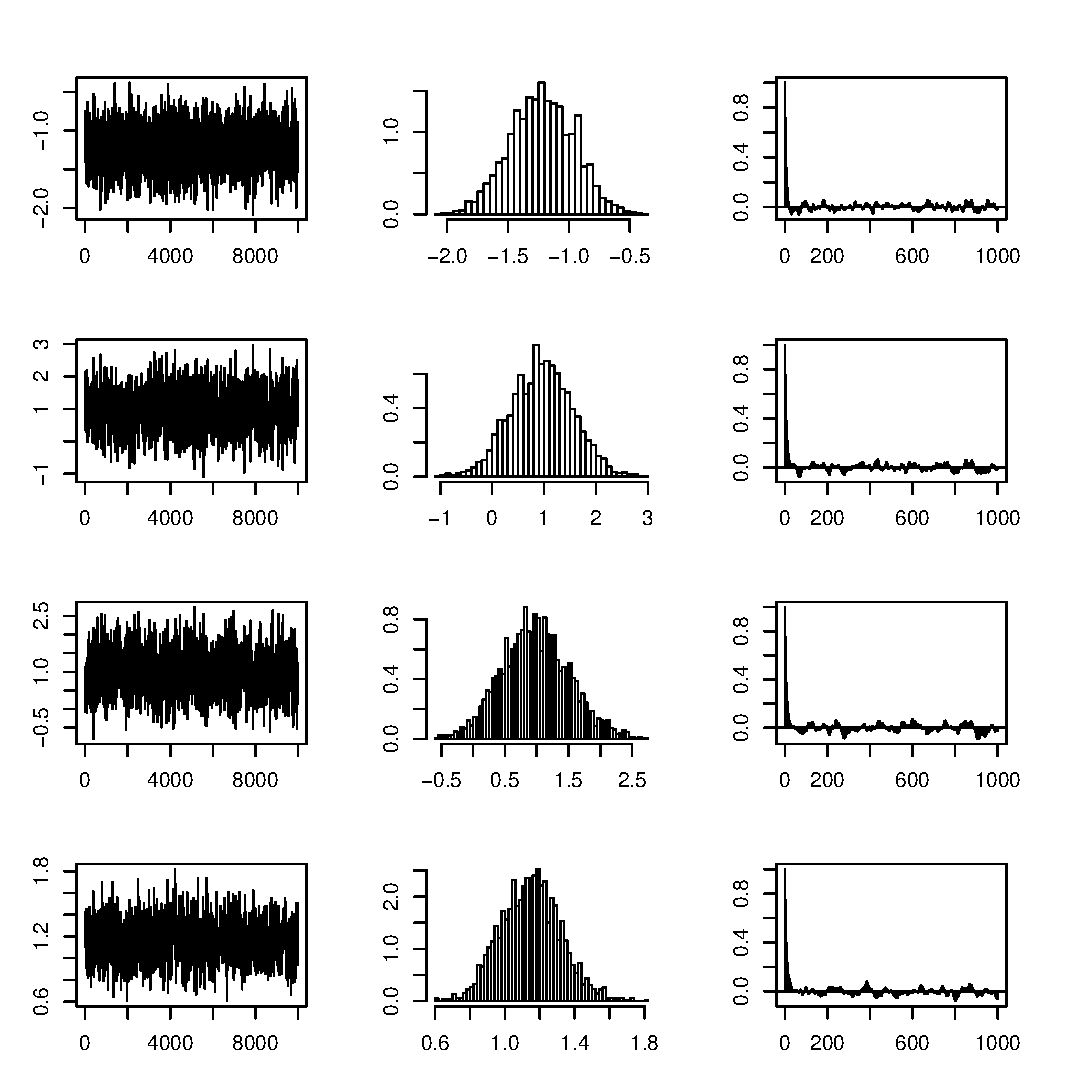
\includegraphics[width=6cm,height=6cm]{figures/hmflatprobit.eps}
\end{columns}
$$
\hat p_i=\Phi\left(-1.2193x_{i1}+0.9540x_{i2}+0.9795x_{i3}+ 1.1481x_{i4}\right).
$$

\end{slide}\begin{slide}
\slidetitle{G-priors for probit models}

Flat prior on $\beta$ inappropriate for comparison purposes
and Bayes factors. 

\pause Replace the flat prior with a hierarchical prior,
$$
\beta|\sigma^2,X\sim\mathscr{N}_k\left(0_k,\sigma^2(X^\tee X)^{-1}\right)
\quad\text{and}\quad
\pi(\sigma^2|X)\propto \sigma^{\RawSienna{-3/2}} \,,
$$
(almost) as in normal linear regression 

\vs\pause\begin{block}{Warning} 
The matrix $X^\tee X$ is {\em not} the Fisher information matrix
\end{block}

\end{slide}
\begin{slide}
\slidetitle{G-priors for testing}

Same argument as before: while $\pi$ is improper, use of the {\em same}
variance factor $\sigma^2$ in both models
means the normalising constant cancels in the Bayes factor.

\pause
\vs Posterior distribution of $\beta$\footnotesize
\begin{eqnarray*}
\pi(\beta|\by,X) & \propto & |X^\tee X|^{1/2} \Gamma((2k-1)/4)\left(\beta^\tee(X^\tee X)\beta\right)^{-(2k-1)/4}
	\pi^{-k/2} \nonumber \\
               && \times\prod_{i=1}^n\,\Phi( \bx^{i\tee}\beta)^{y_i}\left[1-\Phi(\bx^{i\tee}\beta)\right]^{1-y_i}
\end{eqnarray*}\normalsize
{\em [where $k$ matters!]}

\end{slide}\begin{slide}
\slidetitle{Marginal approximation}

Marginal\footnotesize
\begin{eqnarray*}
f(\by|X) & \propto & |X^\tee X|^{1/2}\,\pi^{-k/2}\Gamma\{(2k-1)/4\} \int \left(\beta^\tee(X^\tee X)\beta\right)^{-(2k-1)/4} \\
&& \quad\times\prod_{i=1}^n\,\Phi(\bx^{i\tee}\beta)^{y_i}\left[1-(\Phi(
\bx^{i\tee}\beta)\right]^{1-y_i}\,\text{d}\,\beta\,,
\end{eqnarray*}
\normalsize approximated by\footnotesize
\begin{align*}
\frac{|X^\tee X|^{1/2}}{\pi^{k/2}M}\,\sum_{m=1}^M &\left|\left|X\beta^{(m)}\right|\right|^{-(2k-1)/2}
\prod_{i=1}^n\,\Phi( \bx^{i\tee}{\beta^{(m)}})^{y_i} \left[1-\Phi(
\bx^{i\tee}{\beta^{(m)}})\right]^{1-y_i}\nonumber\\ &\times
\Gamma\{(2k-1)/4\}\,|\widehat V|^{1/2}(4\pi)^{k/2}\,
e^{\Red{+}({\beta^{(m)}}-\widehat\beta)^\tee \widehat
V^{-1}({\beta^{(m)}}-\widehat\beta)/4}\,,
\end{align*}\normalsize
where 
$$
\beta^{(m)} \sim \mathscr{N}_k(\widehat\beta,2\,\widehat V)
$$
with $\widehat\beta$ MCMC approximation of $\mathbb{E}^\pi[\beta|\by,X]$
and $\widehat    V$ MCMC approximation of $\mathbb{V}(\beta|\by,X)$.

\end{slide}\begin{slide}
\slidetitle{Linear hypothesis}

Linear restriction on $\beta$ 
$$
H_0:R\beta=r
$$
($r\in \mathbb{R}^q$, $R$ $q\times k$ matrix)
where $\beta^0$ is $(k-q)$ dimensional and $X_0$ and $\bx_0$ are linear transforms of $X$ and of $\bx$ of dimensions
$(n,k-q)$ and $(k-q)$. 

\vs Likelihood
$$
\ell(\beta^0|\by,X_0)\propto
\prod_{i=1}^n\,\Phi(\bx_0^{i\tee}\beta^0)^{y_i}
\left[1-\Phi(\bx_0^{i\tee}\beta^0)\right]^{1-y_i}\,,
$$

\end{slide}\begin{slide}
\slidetitle{Linear test}

Associated [projected] $G$-prior
$$
\beta^0|\sigma^2,X_0\sim\mathscr{N}_{k-q}\left(0_{k-q},\sigma^2(X_0^\tee
X_0)^{-1}\right)\, \quad \text{and} \quad \pi(\sigma^2|X_0)\propto
\sigma^{-3/2} \,,
$$

\vs\pause
Marginal distribution of $\by$ of the same type\footnotesize
\begin{eqnarray*}
f(\by|X_0) & \propto & |X_0^\tee X_0|^{1/2} \pi^{-(k-q)/2}\Gamma\left\{\frac{(2(k-q)-1)}{4}\right\} 
	\int \left|\left| X\beta^0\right|\right|^{-(2(k-q)-1)/2} \\
             && \quad\prod_{i=1}^n\,\Phi(\bx_0^{i\tee}\beta^0)^{y_i} \left[1-(\Phi(\bx_0^{i\tee}\beta^0)\right]^{1-y_i}
\text{d}\beta^0\,.
\end{eqnarray*}\normalsize

\end{slide}
\begin{frame}[fragile]
\frametitle{{\sf banknote}}

For $H_0:\beta_1=\beta_2=0$, $B^\pi_{10}=157.73$ [against $H_0$]

\vs Generic regression-like output:
\small
\begin{verbatim}
           Estimate  Post. var.  log10(BF)

X1          -1.1552   0.0631       4.5844 (****)
X2           0.9200   0.3299      -0.2875
X3           0.9121   0.2595      -0.0972
X4           1.0820   0.0287      15.6765 (****)

evidence against H0: (****) decisive, (***) strong,
(**) subtantial, (*) poor
\end{verbatim}
\normalsize

\end{frame}
\begin{slide}\slidetitle{Informative settings}

If prior information available on $p(\bx)$, transform 
into prior distribution on $\beta$ by technique of {\em 
imaginary observations:}

\vs\pause
Start with $k$ different values of the covariate vector, $\tilde \bx^1,\ldots,\tilde \bx^k$

For each of these values, the practitioner specifies 
\begin{itemize}
\item[(i)]  a prior guess $g_i$ at the probability $p_i$ associated with $\bx^i$;
\item[(ii)] an assessment of (un)certainty about that guess given by a number $K_i$ of
equivalent ``prior observations''.
\end{itemize}

\pause
\centerline{{\BurntOrange{\bf On how many imaginary observations did you build this guess?}}}

\end{slide}
\begin{slide}
\slidetitle{Informative prior}

$$
\pi(p_1,\ldots,p_k)\propto \prod_{i=1}^kp_i^{K_ig_i-1}(1-p_i)^{K_i(1-g_i)-1}
$$
translates into {\em [Jacobian rule]}
$$
\pi(\beta)\propto \prod_{i=1}^k\,\Phi(\tilde \bx^{i\tee}
\beta)^{K_ig_i-1}\left[ 1-\Phi(\tilde \bx^{i\tee}
\beta)\right]^{K_i(1-g_i)-1}\phi(\tilde \bx^{i\tee}\beta)
$$

\vs\pause

[Almost] equivalent to using the $G$-prior\footnotesize
$$
\beta\sim\mathscr{N}_k\left(0_k,\left[\sum_{j=1}^k \tilde
\bx^j\tilde \bx^{j\tee}\right]^{-1}\right)
$$\normalsize

\end{slide}
\subsection{The logit model}\begin{slide}
\slidetitle{The logit model}

Recall that [for $n_i=1$]
$$
y_i|\mu_i\sim\mathscr{B}(1,\mu_i),\quad \varphi=1
\quad\text{and}\quad
g(\mu_i)=\left(\frac{\exp(\mu_i)}{1+\exp(\mu_i)}\right).
$$

Thus
$$
\mathbb{P}(y_i=1|\beta)=\frac{\exp(\bx^{i\tee}\beta)}{1+\exp(\bx^{i\tee}\beta)}
$$
with likelihood 
\small$$
\ell(\beta|\by,X)=\prod_{i=1}^n\left(\frac{\exp(\bx^{i\tee}\beta)}{1+\exp(\bx^{i\tee}\beta)}\right)^{y_i}
\left(1-\frac{\exp(\bx^{i\tee}\beta)}{1+\exp(\bx^{i\tee}\beta)}\right)^{1-y_i}
$$\normalsize

\end{slide}\begin{slide}
\slidetitle{Links with probit}

\begin{itemize}
\item usual vague prior for $\beta$, $\pi(\beta)\propto 1$

\pause
\item Posterior given by
$$
\pi(\beta|\by,X) \propto \prod_{i=1}^n\left(\frac{\exp(\bx^{i\tee}\beta)}{1+\exp(\bx^{i\tee}\beta)}\right)^{y_i}
\left(1-\frac{\exp(\bx^{i\tee}\beta)}{1+\exp(\bx^{i\tee}\beta)}\right)^{1-y_i}
$$
{\em [intractable]}

\pause
\item Same Metropolis--Hastings sampler
\end{itemize}
\end{slide}\begin{slide}
\slidetitle{{\sf bank}}

\begin{columns}\column{.4\textwidth}
Same scale factor equal to $\tau=1$: 
slight increase in the
skewness of the histograms of the $\beta_i$'s.

\vs Plug-in estimate of predictive probability of a counterfeit 
\column{.6\textwidth}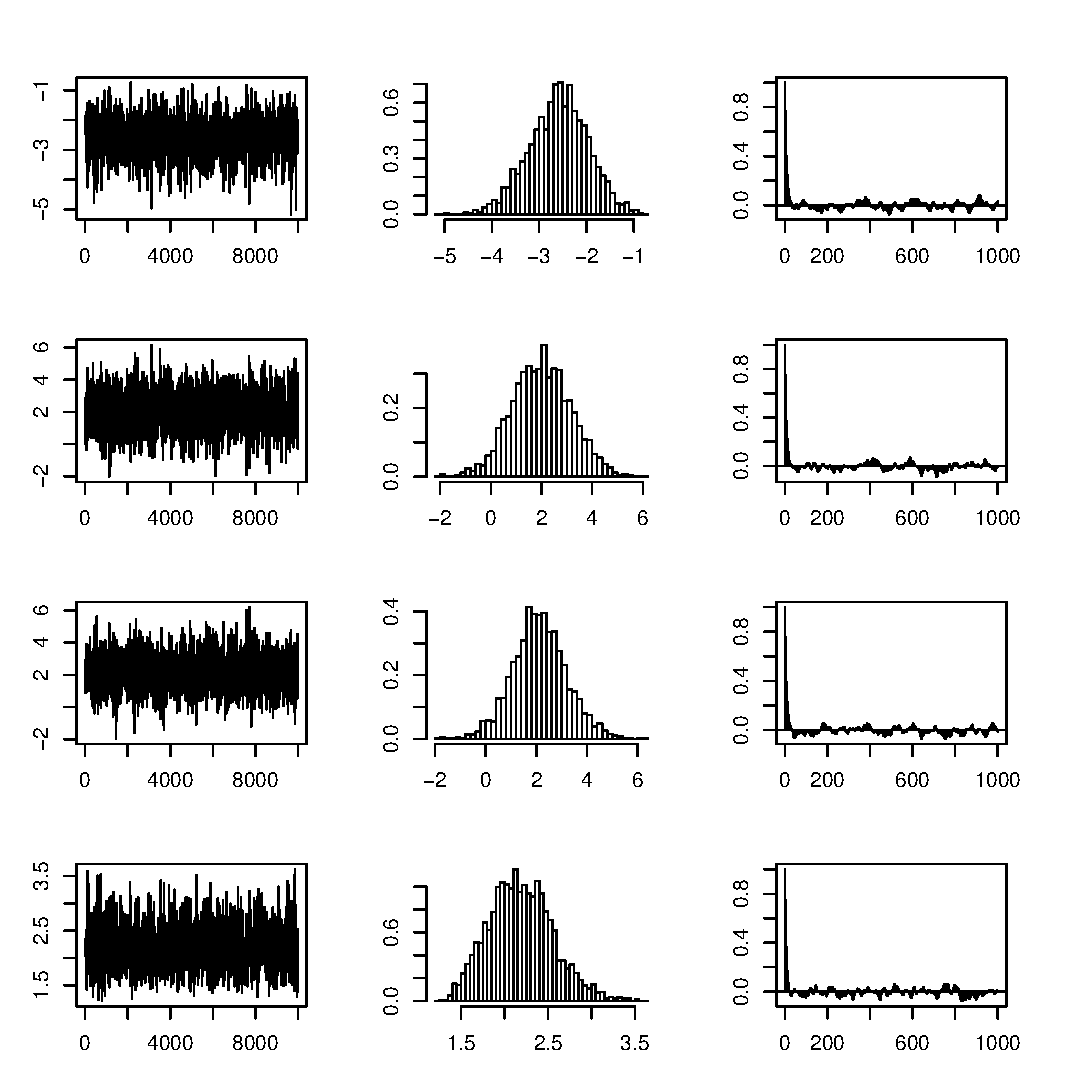
\includegraphics[width=6cm,height=5cm]{figures/hmflatlogit.eps}
\end{columns}
\small$$
\hat p_i=\frac{\exp\left(-2.5888x_{i1}+1.9967x_{i2}+2.1260x_{i3}+
2.1879x_{i4}\right)}{1+\exp\left(-2.5888x_{i1}+1.9967x_{i2}+2.1260x_{i3}+2.1879x_{i4}\right)}.
$$\normalsize

\end{slide}
\begin{frame}[fragile]
\frametitle{G-priors for logit models}

Same story: Flat prior on $\beta$ inappropriate for 
Bayes factors, to be replaced with hierarchical prior,
\small
$$
\beta|\sigma^2,X\sim\mathscr{N}_k\left(0_k,\sigma^2(X^\tee X)^{-1}\right)
\quad\text{and}\quad
\pi(\sigma^2|X)\propto \sigma^{-3/2}
$$

\begin{example}[{\sf bank}]
\begin{verbatim}
           Estimate  Post. var.  log10(BF)

X1          -2.3970   0.3286       4.8084 (****)
X2           1.6978   1.2220      -0.2453
X3           2.1197   1.0094      -0.1529
X4           2.0230   0.1132      15.9530 (****)

evidence against H0: (****) decisive, (***) strong,
(**) subtantial, (*) poor
\end{verbatim}

\end{example}
\normalsize

\end{frame}
\subsection{Loglinear models}
\begin{frame}[label=LLmdL,fragile]
\frametitle{Loglinear models}

\hyperlink{LLintro}{\beamerreturnbutton{Introduction to loglinear models}}
\begin{example}[{\sf airquality}]
Benchmark in {\sf R}\small\\
\verb&   > air=data(airquality)&\\
\normalsize
Repeated measurements over $111$ consecutive days of
ozone $u$ (in parts per billion) and maximum daily temperature $v$ 
discretized into dichotomous variables 
\footnotesize \begin{verbatim}
            month  5  6  7  8  9
 ozone    temp
 [1,31]   [57,79] 17  4  2  5 18
          (79,97]  0  2  3  3  2
 (31,168] [57,79]  6  1  0  3  1
          (79,97]  1  2 21 12  8
\end{verbatim}
\normalsize 
Contingency table with $5\times 2\times 2=20$ entries 
\end{example}

\end{frame}
\begin{slide}\slidetitle{Poisson regression}

Observations/counts $\by=(y_1,\ldots,y_n)$ are integers, so we can choose
$$
y_i\sim\mathscr{P}(\mu_i)
$$
Saturated likelihood
$$
\ell(\mu|\by)=\prod_{i=1}^n\frac{1}{\mu_i!}\mu_i^{y_i}\exp(-\mu_i)
$$

\pause
GLM constraint via log-linear link
$$
\log(\mu_i)=\bx^{i\tee}\beta\,,\quad y_i|\bx^i\sim\mathscr{P}\left(e^{\bx^{i\tee}\beta}\right)
$$

\end{slide}
\begin{slide}\slidetitle{Categorical variables}

\begin{block}{Special feature} {\em Incidence matrix} $X=(\bx^i)$ 
such that its elements are all zeros or ones, i.e.~covariates 
are all indicators/dummy variables!
\end{block}

\vs\pause
Several types of (sub)models are possible depending on relations between categorical variables.

\vs\pause
\begin{block}{Re-special feature} 
Variable selection problem of a specific kind, in the sense that all indicators related
with the {\em same} association must either remain or vanish at once. Thus
much fewer submodels than
in a regular variable selection problem.
\end{block}

\end{slide}
\begin{slide}\slidetitle{Parameterisations}

Example of three variables $1\le u\le I$, $1\le v\le j$ and $1\le w\le K$.

\vs\pause
Simplest non-constant model is
$$
\log(\mu_\tau) = \sum_{b=1}^I \beta^u_b \mathbb{I}_b(u_\tau)
               + \sum_{b=1}^J \beta^v_b \mathbb{I}_b(v_\tau)
               + \sum_{b=1}^K \beta^w_b \mathbb{I}_b(w_\tau)\,,
$$
that is,
$$
\log(\mu_{l(i,j,k)})=\beta^u_i + \beta^v_j +\beta^w_k\,,
$$
where index $l(i,j,k)$ corresponds to $u=i$, $v=j$ and $w=k$. 

\pause Saturated model is 
$$
\log(\mu_{l(i,j,k)})=\beta^{uvw}_{ijk}
$$

\end{slide}\begin{slide}\slidetitle{Log-linear model (over-)parameterisation}

Representation 
$$
\log(\mu_{l(i,j,k)})=\lambda+\lambda^u_i+\lambda^v_j+\lambda^w_k+\lambda^{uv}_{ij}
+\lambda^{uw}_{ik}+\lambda^{vw}_{jk}+\lambda^{uvw}_{ijk}\,,
$$
as in {\sf Anova} models.

\pause
\begin{itemize} 
\item $\lambda$ appears as the overall or reference average effect 
\item $\lambda^u_i$ appears as the marginal discrepancy (against the reference effect $\lambda$) when $u=i$, 
\item $\lambda^{uv}_{ij}$ as the interaction discrepancy (against the added effects $\lambda+\lambda^u_i+
	\lambda^v_j$) when $(u,v)=(i,j)$
\end{itemize}
and so on...

\end{slide}\begin{slide}\slidetitle{Example of submodels}

\small
\begin{enumerate}
\item if both $v$ and $w$ are irrelevant, then
$$
\log(\mu_{l(i,j,k)})=\lambda+\lambda^u_i\,,
$$
\item if all three categorical variables are mutually independent, then
$$
\log(\mu_{l(i,j,k)})=\lambda+\lambda^u_i+\lambda^v_j+\lambda^w_k\,,
$$
\item if $u$ and $v$ are associated but are both independent of $w$, then
$$
\log(\mu_{l(i,j,k)})=\lambda+\lambda^u_i+\lambda^v_j+\lambda^w_k+\lambda^{uv}_{ij}\,,
$$
\item if $u$ and $v$ are conditionally independent given $w$, then
$$
\log(\mu_{l(i,j,k)})=\lambda+\lambda^u_i+\lambda^v_j+\lambda^w_k+\lambda^{uw}_{ik}+\lambda^{vw}_{jk}\,,
$$
\item if there is no three-factor interaction, then
$$
\log(\mu_{l(i,j,k)})=\lambda+\lambda^u_i+\lambda^v_j+\lambda^w_k+\lambda^{uv}_{ij}+\lambda^{uw}_{ik}+\lambda^{vw}_{jk}
$$
{\em [the most complete submodel]}
\end{enumerate}
\normalsize

\end{slide}
\begin{slide}\slidetitle{Identifiability}

Representation 
$$
\log(\mu_{l(i,j,k)})=\lambda+\lambda^u_i+\lambda^v_j+\lambda^w_k+\lambda^{uv}_{ij}
+\lambda^{uw}_{ik}+\lambda^{vw}_{jk}+\lambda^{uvw}_{ijk}\,,
$$
not identifiable but Bayesian approach handles
non-identifiable settings and still estimate properly identifiable quantities. 

\pause
Customary to impose identifiability constraints
on the parameters: set to $0$ parameters corresponding to the first category of
each variable, i.e.~remove the indicator of the first category. 

\vs E.g., if $u\in\{1,2\}$ and $v\in\{1,2\}$, constraint could be
$$
\lambda^u_1=\lambda^v_1=\lambda^{uv}_{11}=\lambda^{uv}_{12}=\lambda^{uv}_{21}=0\,.
$$

\end{slide}
\begin{frame}[fragile]
\frametitle{Inference under a flat prior}

Noninformative prior $\pi(\beta)\propto 1$ gives posterior distribution
\small\begin{eqnarray*}
\pi(\beta|\by,X) &\propto& \prod_{i=1}^n\left\{\exp(\bx^{i\tee}\beta)\right\}^{y_i}\exp\{-\exp(\bx^{i\tee}\beta)\}\\
&=& \exp\left\{ \sum_{i=1}^n y_i\,\bx^{i\tee} \beta - \sum_{i=1}^n \exp (\bx^{i\tee}\beta) \right\}\\
\end{eqnarray*}

\vs\pause
Use of same random walk M-H algorithm as in probit and logit cases, starting with
MLE evaluation
\begin{verbatim}
  > mod=summary(glm(y~-1+X,family=poisson()))
\end{verbatim}

\end{frame}
\begin{slide}\slidetitle{{\sf airquality}}

\begin{columns}\column{.5\textwidth}
Identifiable non-saturated model involves $16$ parameters

Obtained with
$10,000$ MCMC iterations with scale factor $\tau^2=0.5$

\column{.5\textwidth}
\footnotesize
\begin{tabular}{l|r r}
            Effect  & Post. mean  & Post. var. \\
\hline $\lambda$     &  2.8041     & 0.0612 \\
 $\lambda^u_2$       & -1.0684     & 0.2176 \\
 $\lambda^v_2$       & -5.8652     & 1.7141 \\
 $\lambda^w_2$       & -1.4401     & 0.2735 \\
 $\lambda^w_3$       & -2.7178     & 0.7915 \\
 $\lambda^w_4$       & -1.1031     & 0.2295 \\
 $\lambda^w_5$       & -0.0036     & 0.1127 \\
 $\lambda^{uv}_{22}$ &  3.3559     & 0.4490 \\
 $\lambda^{uw}_{22}$ & -1.6242     & 1.2869 \\
 $\lambda^{uw}_{23}$ &- 0.3456     & 0.8432 \\
 $\lambda^{uw}_{24}$ & -0.2473     & 0.6658 \\
 $\lambda^{uw}_{25}$ & -1.3335     & 0.7115 \\
 $\lambda^{vw}_{22}$ &  4.5493     & 2.1997 \\
 $\lambda^{vw}_{23}$ &  6.8479     & 2.5881 \\
 $\lambda^{vw}_{24}$ &  4.6557     & 1.7201 \\
 $\lambda^{vw}_{25}$ &  3.9558     & 1.7128
\end{tabular}
\normalsize
\end{columns}

\end{slide}\begin{slide}\slidetitle{{\sf airquality}: MCMC output}

\begin{columns}\column{.5\textwidth}
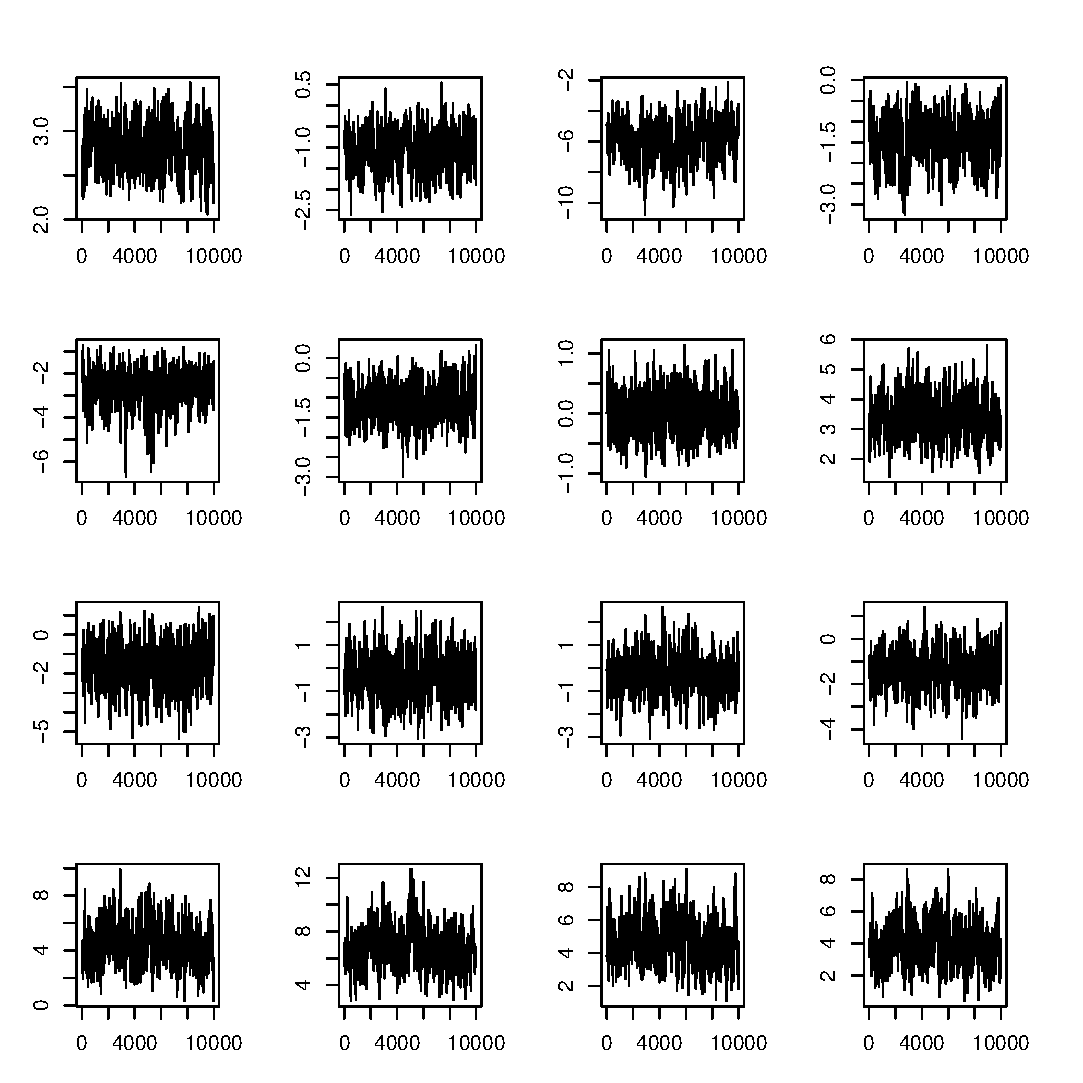
\includegraphics[width=5cm,height=6cm]{figures/trajflatloglin.eps}
\column{.5\textwidth}
\only<2>{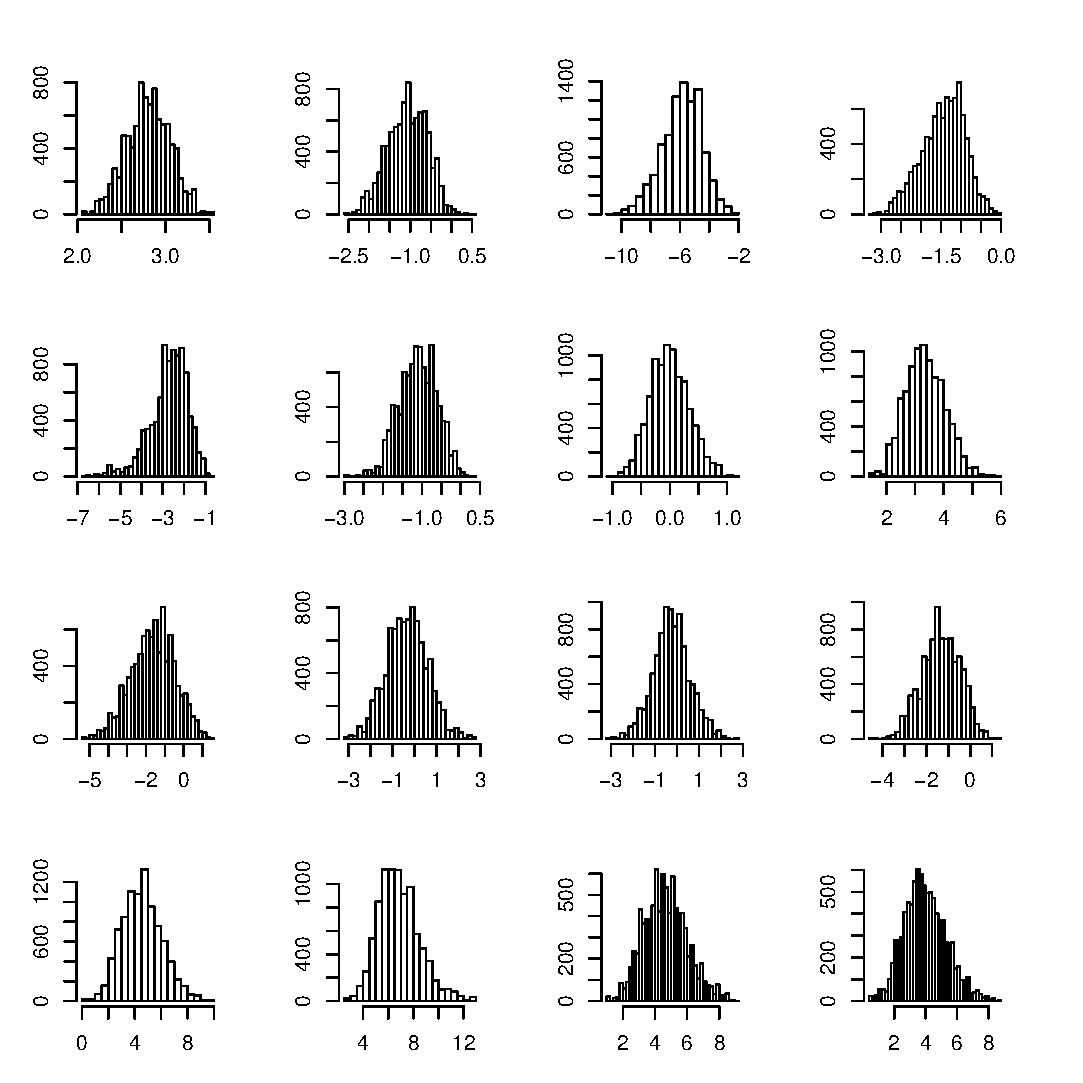
\includegraphics[width=5cm,height=6cm]{figures/histflatloglin.eps}}
\end{columns}

\end{slide}
\begin{frame}
\frametitle{Model choice with $G$-prior}

$G$-prior alternative used for probit and logit models still available:
\begin{eqnarray*}
\pi(\beta|\by,X) & \propto & |X^\tee X|^{1/2}\Gamma\left\{\frac{(2k-1)}{4}\right\}
\left|\left|X\beta\right|\right|^{-(2k-1)/2}\pi^{-k/2} \nonumber \\
&& \quad\times\exp\left\{ \left(\sum_{i=1}^n y_i\,\bx^i\right)^\tee \beta -
\sum_{i=1}^n \exp (\bx^{i\tee}\beta) \right\}
\end{eqnarray*}

\vs\pause
Same MCMC implementation and similar estimates for {\sf airquality}

\end{frame}
\begin{frame}[fragile]
\frametitle{{\sf airquality}}

Bayes factors once more approximated by importance sampling based on normal
importance functions

\vs\pause
\begin{block}{Anova-like output}
\begin{verbatim}
Effect log10(BF)

u:v     6.0983 (****)
u:w    -0.5732
v:w     6.0802 (****)

evidence against H0: (****) decisive, (***) strong,
(**) subtantial, (*) poor
\end{verbatim}
\end{block}

\end{frame}
